\documentclass[conference]{IEEEtran}
\IEEEoverridecommandlockouts
% The preceding line is only needed to identify funding in the first footnote. If that is unneeded, please comment it out.
\usepackage{cite}
\usepackage{amsmath,amssymb,amsfonts}
\usepackage{algorithmic}
\usepackage{graphicx}
\usepackage{textcomp}
\usepackage{xcolor}
\def\BibTeX{{\rm B\kern-.05em{\sc i\kern-.025em b}\kern-.08em
    T\kern-.1667em\lower.7ex\hbox{E}\kern-.125emX}}
\begin{document}

\title{Endless Virtual Data for Machine Learning\\
%{\footnotesize \textsuperscript{*}Note: Sub-titles are not captured in Xplore and
%should not be used}
\thanks{Identify applicable funding agency here. If none, delete this.}
}

\author{\IEEEauthorblockN{1\textsuperscript{st} Christoph Heindl}
\IEEEauthorblockA{\textit{Visual Computing} \\
\textit{PROFACTOR GmbH}\\
4407 Steyr, Austria \\
christoph.heindl@profactor.at}
\and
\IEEEauthorblockN{2\textsuperscript{nd} Sebastian Zambal}
\IEEEauthorblockA{\textit{Machine Vision} \\
\textit{PROFACTOR GmbH}\\
4407 Steyr, Austria \\
sebastian.zambal@profactor.at}
%%%\and
%%%\IEEEauthorblockN{3\textsuperscript{rd} Markus Ikeda}
%%%\IEEEauthorblockA{\textit{Robotics} \\
%%%\textit{PROFACTOR GmbH}\\
%%%4407 Stey, Austria \\
%%%markus.ikeda@profactor.at}
%%%\and
%%%\IEEEauthorblockN{~~~~~~~~~4\textsuperscript{th} Christian Eitzinger~~~~~~~~~}
%%%\IEEEauthorblockA{\textit{Machine Vision} \\
%%%\textit{PROFACTOR GmbH}\\
%%%4407 Stey, Austria \\
%%%christian.eitzinger@profactor.at}
%%%\and
%%%\IEEEauthorblockN{5\textsuperscript{th} Andreas Pichler}
%%%\IEEEauthorblockA{\textit{Robotics} \\
%%%\textit{PROFACTOR GmbH}\\
%%%4407 Stey, Austria \\
%%%anreas.pichler@profactor.at}
\and
\IEEEauthorblockN{6\textsuperscript{th} Josef Scharinger}
\IEEEauthorblockA{\textit{Institute of Computational Perception} \\
\textit{Johannes Kepler University}\\
4040 Linz \\
josef.scharinger@jku.at}
}

\maketitle

\begin{abstract}
Impressive results have been achieved in computer vision via machine learning methods over the last years. However, for many highly specialized industrial applications these methods cannot directly be applied due to the lack of large amounts of training data. In this paper we propose a software framework that provides artificial data. Such artificial data opens the door for machine learning even when it is hard or impossible to acquire real data. The presented system is flexible in the sense that it supports image data generation in a flexible way. We show how artificial images can directly be used in pytorch to perform deep neural network training. 
\end{abstract}

\begin{IEEEkeywords}
machine learning, artificial data, data augmentation
\end{IEEEkeywords}

\section{Introduction}

TODO: Write some good introduction, cite related work such as \cite{2017_Varhegyi_visualServoingRGBD} and \cite{2017_Johnson_DrivingInTheMatrix}...

\begin{figure}[htbp]
\centerline{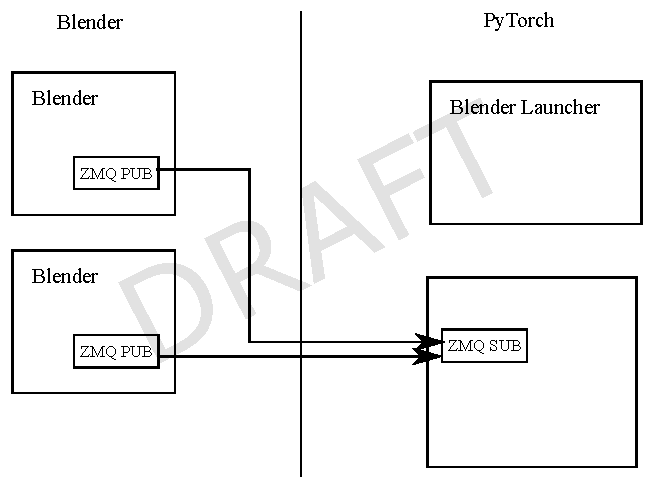
\includegraphics[width=\columnwidth]{figures/architecture/architecture.pdf}}
\caption{\label{fig:architecture} Architecture of our system: Individual instances generate artificially rendered images (left). These are consumed in a pytorch environment for training of deep neural networks (right).}
\label{fig}
\end{figure}


\begin{figure}[htbp]
\centerline{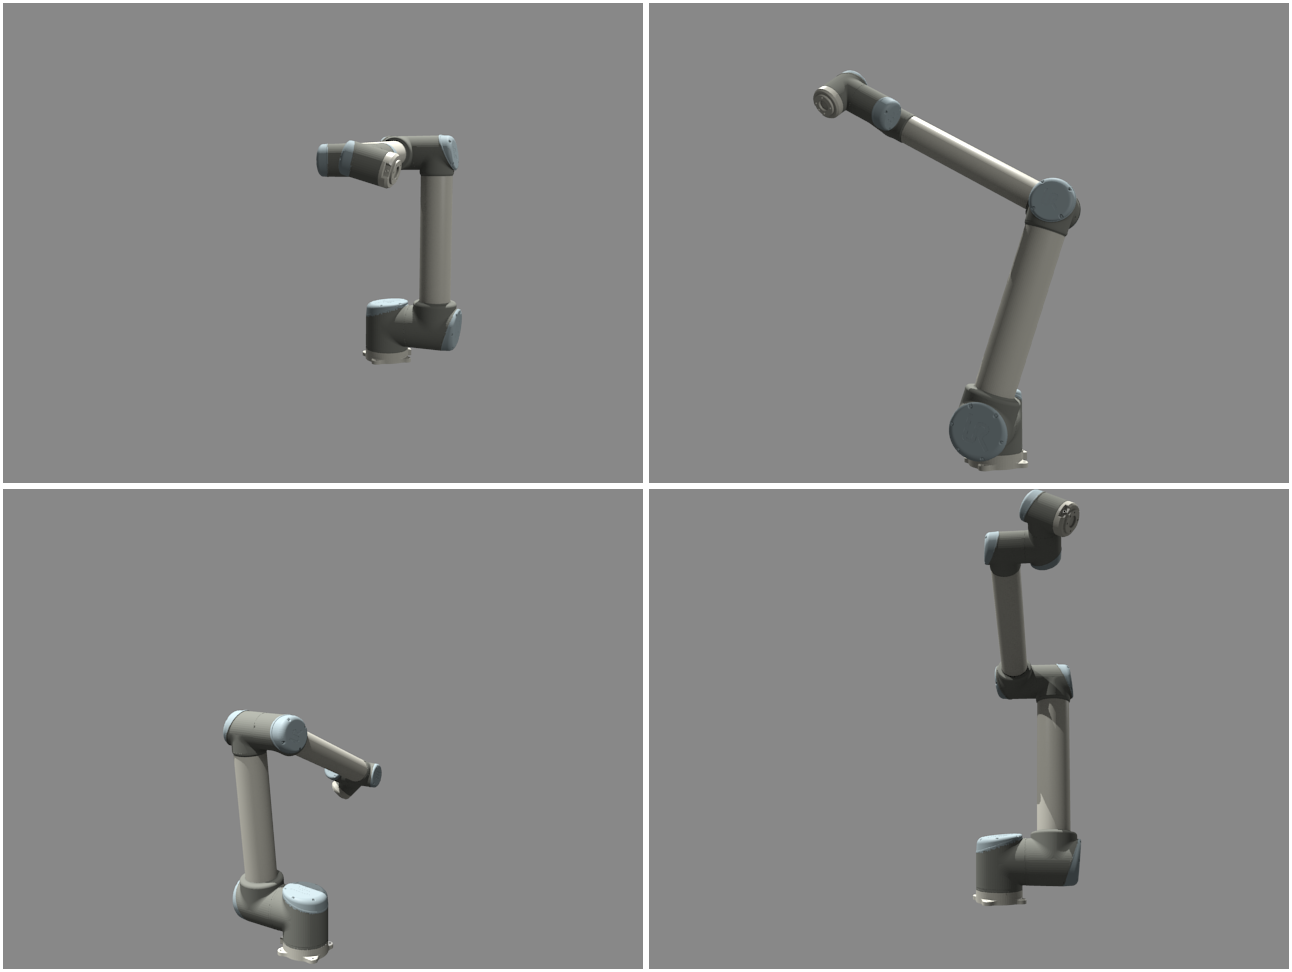
\includegraphics[width=\columnwidth]{figures/examplesUR10/renderedImages.png}}
\caption{\label{fig:architecture} Architecture of our system: Individual instances generate artificially rendered images (left). These are consumed in a pytorch environment for training of deep neural networks (right).}
\label{fig}
\end{figure}


\section{Method}

\subsection{3D Scene Rendering}

TODO: Outline Python-support of Blender, Explain scripting in Blender, creation of meta-data (joint locations, etc.)...

\subsection{Data Loaders for Deep Learning}

TODO: Explain basic concepts of PyTorch and DataLoaders, etc.

\subsection{System Integration}

TODO: Explain how Blender and pytorch are linked with ZMQ, publish/subscribe, ...

\section{Results}

TODO

\begin{table}[htbp]
\caption{Performance evaluation}
\begin{center}
\begin{tabular}{|c|c|}
\hline
\textbf{Blender instance} & \textbf{Runtime ms/batch} \\
\hline
1 & 103 ms ± 5.17 ms \\
\hline
2 & 43.7 ms ± 10.3 ms \\
\hline
\end{tabular}
\label{tab1}
\end{center}
\end{table}

\section*{Acknowledgment}

Work presented in this paper has received funding from the European Union’s Horizon 2020 research and innovation programme under grant agreement No 721362 (project “ZAero”).

\small
\bibliographystyle{ieeetr}
\bibliography{biblio}



%%%\begin{thebibliography}{00}
%%%\bibitem{b1} G. Eason, B. Noble, and I. N. Sneddon, ``On certain integrals of Lipschitz-Hankel type involving products of Bessel functions,'' Phil. Trans. Roy. Soc. London, vol. A247, pp. 529--551, April 1955.
%%%\bibitem{b2} J. Clerk Maxwell, A Treatise on Electricity and Magnetism, 3rd ed., vol. 2. Oxford: Clarendon, 1892, pp.68--73.
%%%\bibitem{b3} I. S. Jacobs and C. P. Bean, ``Fine particles, thin films and exchange anisotropy,'' in Magnetism, vol. III, G. T. Rado and H. Suhl, Eds. New York: Academic, 1963, pp. 271--350.
%%%\bibitem{b4} K. Elissa, ``Title of paper if known,'' unpublished.
%%%\bibitem{b5} R. Nicole, ``Title of paper with only first word capitalized,'' J. Name Stand. Abbrev., in press.
%%%\bibitem{b6} Y. Yorozu, M. Hirano, K. Oka, and Y. Tagawa, ``Electron spectroscopy studies on magneto-optical media and plastic substrate interface,'' IEEE Transl. J. Magn. Japan, vol. 2, pp. 740--741, August 1987 [Digests 9th Annual Conf. Magnetics Japan, p. 301, 1982].
%%%\bibitem{b7} M. Young, The Technical Writer's Handbook. Mill Valley, CA: University Science, 1989.
%%%\end{thebibliography}
%%%\vspace{12pt}
%%%\color{red}
%%%IEEE conference templates contain guidance text for composing and formatting conference papers. Please ensure that all template text is removed from your conference paper prior to submission to the conference. Failure to remove the template text from your paper may result in your paper not being published.

\end{document}
